\documentclass[12pt]{report}

\usepackage{color}
\usepackage[english]{babel}
\usepackage[utf8]{inputenc}
\usepackage{graphicx}
\usepackage{verbatim}
\usepackage{listings}
\usepackage{url}
\usepackage{stringenc}
\usepackage{pdfescape}
\usepackage{subfig}
\usepackage{float}
\usepackage{csquotes}  
\usepackage{tabularx}  
\usepackage[toc,page]{appendix}
\usepackage{caption}
\usepackage{titlesec}
\titleformat{\chapter}{\normalfont\huge}{\thechapter.}{20pt}{\huge\bf}

\setcounter{secnumdepth}{3}
\setcounter{tocdepth}{3} 

\begin{document}
\setlength{\textwidth}{16cm}
\setlength{\textheight}{22cm}
\title{\huge{\textbf{\textit{aWareHouse}}}\linebreak
\Large\textbf{\\Environment Control System for Warehouses}\linebreak\linebreak\linebreak

\includegraphics[width=8cm]{feup.pdf}\linebreak \linebreak
\large{MSc in Informatics and Computer Engineering} \linebreak
\large{Programming Paradigms \\ EIC0065-2S}\linebreak
}
\author{
Duarte Nuno Pereira Duarte - 201109179 (ei11101@fe.up.pt)\\
Hugo José Freixo Rodrigues - 201108059 (ei11086@fe.up.pt)\\
João Pedro Matos Teixeira Dias - 201106781 (ei11137@fe.up.pt)\\
\\
\\ Faculdade de Engenharia da Universidade do Porto \\ Rua Roberto Frias, s\/n, 4200-465 Porto, Portugal
 \vspace{1cm}}
%\date{Junho de 2007}
\maketitle
\thispagestyle{empty}

%************************************************************************************************
%************************************************************************************************

\newpage
\section*{Abstract}

We are in the rise of IoT (Internet of things). A world were everything is connected and we can, with simple tools, monitory and control everything. In this context, there is a lot of space for a more recurrent use of different programming paradigms because of the need of interaction with different layers of system architecture for a single application, since hardware to web.

Our application, \textit{aWareHouse}, was designed with the objective of, with a simple interface, we can monitory a house or a warehouse in terms of environment conditions (temperature, humidity, sound and luminosity). 

For accomplishing this was used a combination of hardware/software and some different programming languages, in a way that gave us a stable application that can be used for setting a alarm system when occurs changes in our environment, for taking decisions analysing the past conditions and the relations with external (meteorological) conditions or simple look at the current conditions inside our warehouse.


\newpage
%************************************************************************************************
%************************************************************************************************
\tableofcontents
%************************************************************************************************
%************************************************************************************************
\newpage

\chapter{Introduction}

The \textit{aWareHouse} project was developed for the Programming Paradigms course unit of the Master in Informatics and Computing Engineering at FEUP. The project was developed with the objective of combine, at least, three programming paradigms in the same application.

The base motivation for this project was the Internet of Things, as defined by \textit{Gartner}:

\blockquote{The Internet of Things (IoT) is the network of physical objects that contain embedded technology to communicate and sense or interact with their internal states or the external environment.}

So, we designed a low cost system capable of giving the user the possibility of, using a relative small hardware box, monitory the environment of a given place like a home or warehouse. This, associated with a system capable of maintain records of the past conditions of the environment (plus external weather conditions), results in one application that gives the user the capacity of taking decision, be aware of the environment status using alerts and see the current conditions.

As explained before the capabilities of this application make this a system useful in a lot of situations, for example, the monitoring of a warehouse and verify the relation between weather and internal conditions to make decision on what is the best settings for a refrigeration system and assure that the, for example, temperature is always below the maximum recommended. Other example is simple use it as a house control system and, for example, verify if someone forgot to turn any light off.

\newpage
\chapter{System Description}
\section{Conceptual Description}
\subsection{Functionalities}

\begin{figure}
    \centering
    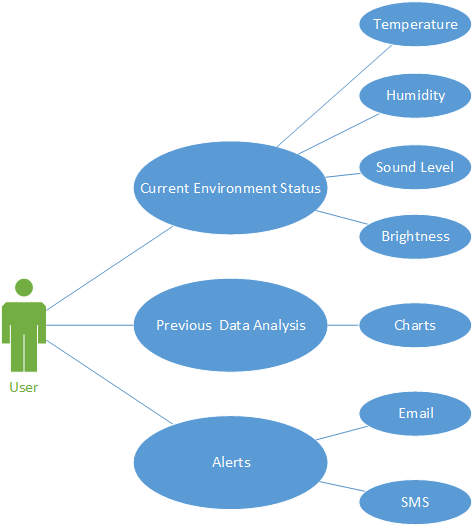
\includegraphics[scale=0.5]{use.png}
    \caption{Use Case diagram.}
    \label{fig:use}
\end{figure}

The \textit{aWarehouse} application consist in a system that scans the environment of the room where the sensors are placed and stores all the information about it on a database.

The system can read temperature, humidity, sound and luminosity values as described in \ref{fig:use}. Additionally user can define maximum and minimum values so the system will alert whenever an environment factor exceeds this range.
This way the user can have absolute control of the room where \textit{aWarehouse} is installed. This application can be very useful in a server room, with the temperature sensor the user can control the room temperature and prevent an overheating. With the sound sensor the user knows if someone is in the room and with the luminosity sensor the user can check if,for example, a door is open.



\subsection{Architecture}

\subsubsection{Physical Architecture}

\begin{figure}[H]
    \centering
    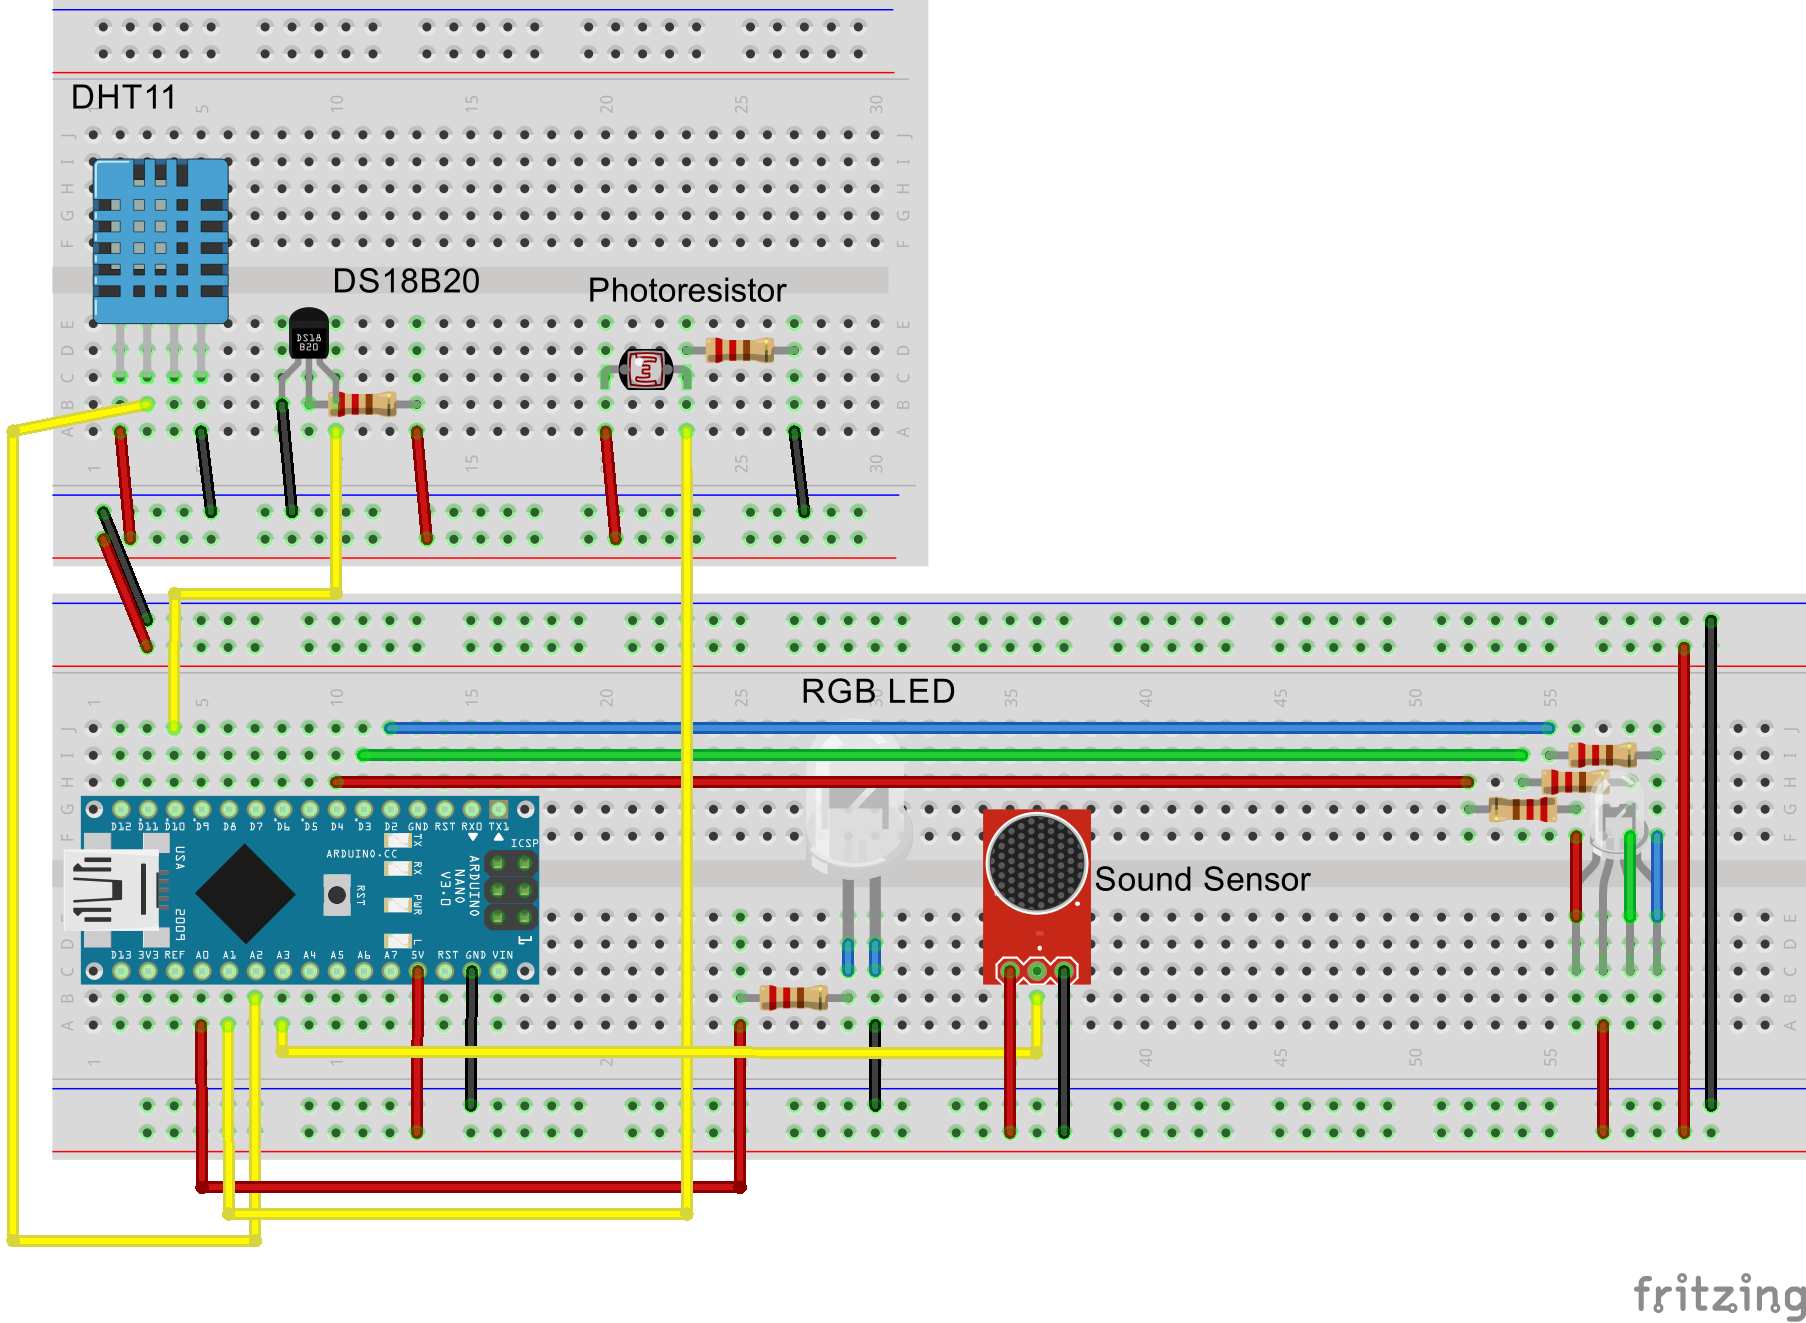
\includegraphics[width=0.8\textwidth]{schematics.png}
    \caption{Circuit diagram.}
    \label{fig:circ}
\end{figure}

\begin{table}[H]
\begin{tabularx}{0.85\textwidth}{ |l|X|p{3cm}| }
  	\hline
  	\textbf{Sensor}  & \textbf{Description} & \textbf{Input/Output} \\
 	\hline
 	DHT11  & Basic and low-cost digital temperature and humidity sensor. It uses a capacitive humidity sensor and a thermistor to measure the surrounding air, and spits out a digital signal on the data pin. & Temperature and Humidity values. \\
 	\hline
 	DS18B20  & 1-wire digital temperature sensor fairly precise (+- 0.5ºC over much of the range) and can give up to 12 bits of precision from the onboard digital-to-analog converter. & Temperature values. \\
 	\hline
 	LM393 & One single channel output sound level. Low level output signal and when there is sound output low, lights lit. & Sound level values. \\
 	\hline
 	Diffused LED & A diffuse LED with with separate red, green and blue LED chips inside, capable of emitting a color-mix resulted of the values passed to each chip. & RGB Color or Color-Mix.\\
 	\hline
 	Photo cell & Photo cell or CdS photoresistor is a little light sensor. As the squiggly face is exposed to more light, the resistance goes down and the voltage goes up. & Voltage value.\\
 	\hline
\end{tabularx}
	\caption{Sensors description.}
  	\label{tab:prolangs}
\end{table}

\textbf{\\Arduino}

\begin{figure}[H]
    \centering
    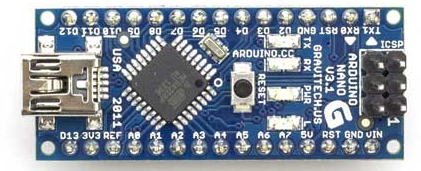
\includegraphics[width=0.5\textwidth]{img/arduino.png}
    \caption{Arduino micro-controller.}
    \label{fig:arduino}
\end{figure}

The Arduino Nano (fig.\ref{fig:arduino}) is a small, complete, and breadboard-friendly micro-controller based on the ATmega328 processor chip and works with a Mini-B USB cable for energy and data transfer. It has 32 KB of flash memory space of which 2 KB used by bootloader.

Each of the 14 digital pins on the Nano can be used as an input or output and 8 analog inputs, each of which provide 10 bits of resolution (i.e. 1024 different values). 

The Arduino provides an UART TTL (5V) serial communication, which is available on digital pins 0 (RX) and 1 (TX). An FTDI FT232RL on the board channels this serial communication over USB and the FTDI drivers (included with the Arduino software) provide a virtual COM port to software on the computer. 


\textbf{\\Raspberry Pi}

\begin{figure}[H]
    \centering
    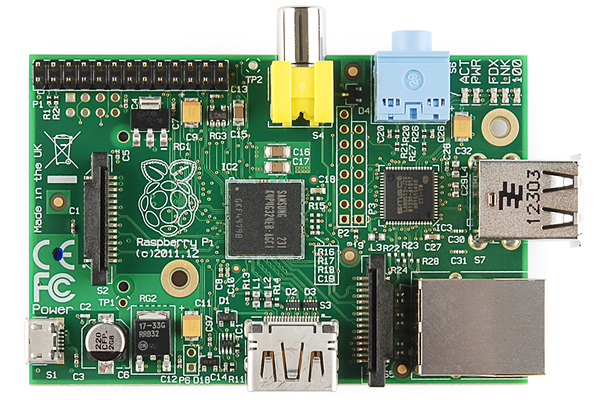
\includegraphics[width=0.5\textwidth]{img/rpi.png}
    \caption{Raspberry Pi 1 Model B.}
    \label{fig:rpi}
\end{figure}

The \textit{Raspberry Pi 1 Model B} (fig. \ref{fig:rpi}) is a single-board computer which can be used for many of the things that a desktop is used to.

The design is based around a Broadcom BCM2835 SoC, which includes an ARM1176JZF-S 700 MHz processor, VideoCore IV GPU, and 512 Megabytes of RAM. The memory used is a SD card for booting and long-term storage. This board is intended to run Linux kernel based operating systems. Additionally this has two USB ports and a 10/100 Ethernet controller.

\subsubsection{Logic Architecture}

\begin{figure}[H]
    \centering
    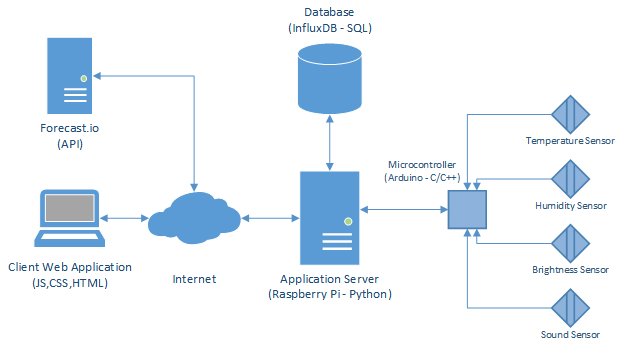
\includegraphics[width=0.9\textwidth]{arc.png}
    \caption{Architecture diagram.}
    \label{fig:arc}
\end{figure}

\subsection{Programming Languages and Technologies}

In the context of realizing this project it was conciliated a diversity of technologies and programming languages that, working together in the architecture presented at fig. \ref{fig:arc}, made the application possible. Starting by enumerating the programming languages used and the reasons for choosing those languages is presented in the table \ref{tab:prolangs}.


\begin{table}[H]
\begin{tabularx}{0.8\textwidth}{ |l|X| }
  	\hline
  	Arduino  & C/C++  \\
 	\hline
 	Python  & item 2   \\
  	\hline
 	Web Languages  & HTML,JS,CSS   \\
	\hline
	SQL  & InfluxDB   \\
	\hline
\end{tabularx}
	\caption{Programming languages.}
  	\label{tab:prolangs}
\end{table}

In addiction to the programming languages we used a set of technologies as a part of our application as presented in table \ref{tab:tech}.

\begin{table}[H]
\begin{tabularx}{0.8\textwidth}{ |l|X| }
  	\hline
  	InfluxDB  &   \\
 	\hline
 	Grafana  &   \\
  	\hline
 	Web API's & Twilio, Mandrill, Forecast.io   \\
	\hline
\end{tabularx}
	\caption{Technologies.}
  	\label{tab:tech}
\end{table}

-Python lib's (?)

-Arduino lib's (?)

\section{Implementation Description}

\subsection{Implementation Details}

Socket communication over usb (Python - Arduino (c/c++))

HTTP REST protocol  (web application - python server - InfluxDB - external API's - JSON)

\subsection{Development Environment}

Raspberry Pi, Arduino, Arduino IDE  + Compiler, Atom, SSH, Python Compiler, ARM architecture , Version Control - Git

\newpage
\chapter{Conclusion}

almost ready to market (?), easy to expand or adapt, usefulness of programming paradigms, big data and internet of things

\newpage
\chapter{Improvements}

Motion, better management of storage (slow), advice system (?), better safety (credentials)
\newpage
\chapter{Resources}
\section{\it{Bibliography}}
\begin{description}
\item Visual Studio 2013 Ultimate, Microsoft, \url{http://www.visualstudio.com/}.
\end{description}
\section{\it{Software}}
\begin{description}
\item Visual Studio 2013 Ultimate, Microsoft, \url{http://www.visualstudio.com/}.
\end{description}

\newpage

\begin{appendices}
\chapter{Appendix}
\section{Hardware}
\subsection{Raspberry Pi}

Chip Broadcom BCM2835 SoC full HD multimedia applications processor

CPU 700 MHz Low Power ARM1176JZ-F Applications Processor

GPU	Dual Core VideoCore IV® Multimedia Co-Processor
	  	
Memory 512MB SDRAM

Ethernet onboard 10/100 Ethernet RJ45 jack

USB 2.0 Dual USB Connector

Video Output HDMI (rev 1.3 \& 1.4) Composite RCA (PAL and NTSC)

Audio Output 3.5mm jack, HDMI

Onboard Storage SD, MMC, SDIO card slot

Operating System Linux

Dimensions 8.6cm x 5.4cm x 1.7cm
\subsection{Arduino}

Specifications:

Microcontroller	Atmel ATmega328

Operating Voltage (logic level)	5 V

Input Voltage (recommended)	7-12 V

Input Voltage (limits)	6-20 V

Digital I/O Pins	14 (of which 6 provide PWM output)

Analog Input Pins	8

DC Current per I/O Pin	40 mA

Flash Memory	32 KB (ATmega328) of which 2 KB used by bootloader

SRAM  2 KB (ATmega328)

EEPROM	1 KB (ATmega328)

Clock Speed	16 MHz

Dimensions	0.73" x 1.70"

Length	45 mm

Width	18 mm

Weigth	5 g

\subsection{Sensor DHT11}
Technical specs:
\begin{itemize}
\item Low cost
\item  3 to 5V power and I/O
\item   2.5mA max current use during conversion (while requesting data)
\item  Good for 20-80\% humidity readings with 5\% accuracy
 \item   Good for 0-50C temperature readings +- 2C accuracy
 \item   No more than 1 Hz sampling rate (once every second)
 \item   Body size 15.5mm x 12mm x 5.5mm
 \item   4 pins with 0.1" spacing

    \end{itemize}

\subsection{Sensor DS18B20}
Technical specs:
\begin{itemize}
\item Usable temperature range: -55 to 125 C (-67F to +257F)
\item 9 to 12 bit selectable resolution
\item Uses 1-Wire interface- requires only one digital pin for communication
\item Unique 64 bit ID burned into chip
\item Multiple sensors can share one pin
\item +-0.5C Accuracy from -10C to +85C
\item Temperature-limit alarm system
\item Query time is less than 750ms
\item Usable with 3.0V to 5.5V power/data
\end{itemize}
\subsection{Sound Sensor (LM393)}
Technical specs:
\begin{itemize}
\item LM393 (?)
\item Electret microphone
\item Working voltage: DC 4 ~ 6 V
\item With a signal output instruction
\item One single channel output
\item Low level output signal
\item When there is sound output low, lights lit
\end{itemize}
\subsection{Diffused Led}
Technical specs:
\begin{itemize}
\item 10mm diameter
\item Red: 623 nm wavelength, Green: 523 nm, Blue: 467 nm
\item Red: 1.8-2.2V Forward Voltage, at 20mA current, Green: 3.0-3.4V, Blue: 3.0-3.4V
\item 50 degree viewing angle.
\item Red: 700 mcd typical brightness, Green: 2100 mcd, Blue: 900 mcd
\end{itemize}
\subsection{Photo cell (CdS photoresistor)}
Technical specs:
\begin{itemize}
\item When its light, the resistance is about 5-10KOhm, when dark it goes up to 200KOhm.
\item The voltage on the pin will be 2.5V or higher when its light out and near ground when its dark.
\end{itemize}
\end{appendices}

\end{document}
